\begin{fullwidth}
\chapter{\label{ch:nba_intro}
The Neural Blackboard Architecture applied to language}
\end{fullwidth}

\begin{chabstract}

In this chapter we introduce...

\end{chabstract}


\section{Introduction}

{\label{931947}}

Human languages rely on composition operations at several levels of representations: phonemes combine into morphemes which combine into words which themselves combine into 
phrases and sentences. For example, in Chomsky's Minimalist Program for Syntax \citep{Chomsky_2013}, the center stage is given to `Merge', the operation which combines words and phrases to create larger phrases.

Proposing a satisfactory neural model for the ``composition'' operations required by language is linked to solving the binding problem \citep{marcus14}.
The term binding was introduced into the neuro-scientific community by von der Malsburg\citep{von_der_Malsburg_1994} during the first explorations of neural phase synchronization for ``variable binding'', which is a term taken literally from computer science, meaning to link a data structure to a name so it can be later accessed by that name.
Binding is also motivated by the empirical discovery of the distributed and segmented encoding of features along the cortex. For example color and shape, in the case of vision, are robustly integrated during perception but can be independently impaired by brain damage.

The general binding problem actually comprises four different sub problems, namely~\emph{General Coordination},~\emph{Feature-Binding},~\emph{Variable Binding} and the~\emph{Subjective Unity of Perception}\citep{Feldman_2012}.
The current work is specifically motivated by the~\emph{Variable Binding} sub-problem that is presented by Feldman as an abstract high level cognitive faculty, mainly required by symbolic thought, to bind values to instances of variable types that form part of a structured representation.
In this respect, it is a function that arises mostly in human languages and goes beyond the extensively studied sensory, attention and short-term memory phenomena of feature binding, that only require linking features exclusively, in a bag, to avoid confusion with simultaneous representations, like a red circle and a blue square presented side by side in a screen.

~\emph{Variable binding} is illustrated by the capacity to run logical inference on data structures that encode relationships between their items.
For example the sentence ``\emph{Mary owns a book}" allows to establish a relation of the type \emph{own(Mary, book)} that implies \emph{owner(book, Mary)}, such that we can later ask the question ``\emph{Who owns this book?}'', which would not be answerable under a simpler feature binding mechanism that would just confuse the three words in a bag as just belonging to the same sentence.
To implement this in language, most linguistic theories propose that there are types of words, named grammatical categories, like 'noun' and 'verb', that are instantiated during sentence comprehension to be combined under a finite set of constraints.
These instantiated word types would point to each other to form a graph data structure, a tree, on which query and join operations can be performed, and they would also point to their corresponding specific words.
Then solving ~\emph{Variable binding} in language, requires a biologically feasible implementation of a pointer mechanism that can link instantiated grammatical categories and their corresponding words, which we will demonstrate with the Neural Blackboard Architecture.


\subsection{Some language neuroimaging studies of binding}
{\label{intro:imaging}}

Most linguistic theories assume a constituency property that allows to combine and replace smaller phrases in larger phrases.
Since solving variable binding requires an explanation of how to implement links between bits of information - like words and word types - to create basic data structures, like phrases in language, it is likely to also explain how to create links between such basic structures.

Behavioral evidence for constituents in phrases has been around for a while\citep{bever1969underlying, abrams1969syntactic}, with more recent studies demonstrating the reuse of 
recently heard syntactic structures through syntactic priming experimental paradigms\citep{bock2007persistent, branigan2000syntactic}.
But only recently we have started to characterize the detailed neural correlates of constituency and word binding with diverse brain-imaging techniques
\citep{Nelson_2017, fedorenko2016neural, brennan2016abstract, ding2016cortical, bemis2012basic, Pallier_2011, bastiaansen2010syntactic, longe2006grammatical}.

We selected The ECoG analysis of Nelson et al.\citep{Nelson_2017} as the first study to compare to our model.
It is one of the only two studies so far demonstrating spatially specific and temporally detailed neural dynamics of phrase processing, 
made possible by analyses of intracranial neurophysiological data taken from epileptic patients.
Moreover it is the first one to characterize the specific patterns of phrase-structure formation, possibly revealing the first neural signatures of variable binding 
related operations. Nelson et al. refer to them as "merge" operations that combine syntactic objects (word types and phrase types).
In the study words were presented sequentially to patients in a screen to be read under a Rapid Serial Visual Presentation paradigm.
The task was to keep a phrase of up to 10 words in memory to compare it just after with a probe sentence composed of 2 to 5 words.
We will show that simulation of the NBA portion responsible for variable binding, while only tuned for correct operation, generates strikingly similar temporal patterns of 
neural activity when aggregating the binding operations corresponding to complete phrase processing, assuming the phrase grammar and bottom-up parsing scheme employed by 
Nelson et al. in their analyses.

As a second study, we selected an fMRI experiment \citep{Pallier_2011} to portray the capacity of the model to capture results from multiple neuroimaging spatio-temporal scales.
In this experiment, trials with lists of 12 words obtained by concatenating phrases of a given length, were presented to healthy subjects.
Conditions were formed from all combinations of m by n that give 12, satisfying the form n phrases of m words, like 2 phrases of 6 words.
Besides normal words, the design also included pseudoword conditions that maintained morphological markers and closed-class (function) words.
This allowed the authors to demonstrate a clear separation of syntactic and semantic binding neural activation patterns in language related regions, which is interesting to us, 
since syntactic specific patterns are the closest to the abstract considerations of binding of our model, assuming the same phrase grammar and parsing scheme employed for 
comparison with the ECoG results.
The authors found a sub-linear pattern of neural activation as the number of constituents increase, which could not be explained by a simple "accumulation" model motivated by 
measurements of sequence learning tasks in awake macaque monkeys.
The Neural Blackboard Architecture predicts this sub-linear effect from the circuit recruitment process required by the number of binding operations, 
alongside expected patterns of hemodynamic peak onset differences from delay activity considerations.


\subsection{Neural models of language}

{\label{619233}}

To understand how the cognitive faculty of language operates, we need to take into account, not only the underlying supporting structures, but also their dynamics. 
This means that we have to consider simultaneously the grammars given by linguistic theory and a temporal component to give birth to computational mechanisms, like 
automaton models, capable of explaining behavior\citep{hale2014automaton}.
To extend this into neuroscience we have to go even further and also provide reasonable implementation models, corresponding to the biological components of the brain.
This implementation is necessary to be able to go beyond behavioral measurements and ultimately test computational hypotheses directly against the currently available spatio-temporal neural measurements.

A good example of success in this direction is the computational~theory of visual receptive fields\citep{lindeberg2017normative} which has made impressively accurate predictions 
about the shape of the biological visual fields in the retina.
Knowledge of these basic units of visual perception has even recently allowed to correlate the mechanisms behind deep convolutional neural networks to visual 
pathways\citep{Guclu_2015,Eickenberg_2017} and has influenced our understanding of higher-level visual phenomena such as visual illusions\citep{Eagleman_2001}.
Although expecting at the moment something similar in the case of language might sound overambitious, we must note that basic phonetic features have already been decoded in the 
Superior Temporal Gyrus from electrocorticography (ECoG)\citep{Mesgarani_2014}.
Moreover, as presented in the previous section, recently several spatial and temporal detailed neural correlates of constituency and binding have been revealed.

Numerous Artificial Neural Networks (ANNs) have been implemented, motivated by biological principles in the brain, to model particular aspects of brain language function or to reproduce behavior in specific language tasks.
Nonetheless they lack dynamic biological considerations necessary to match their output with neuroimaging measurements, and except for Vector Symbol Architectures (VSA)\citep{smolensky2006harmonic}, they are difficult to integrate into a general framework for the implementation of the complete language function.

For an extensive review of these models, categorized by language function, we recommend reading Bocancia\citep{bocancia2014psycholinguistically}, 
Christiansen et al.\citep{Christiansen_1999} and Miikkulainen\citep{miikkulainen1997natural}.
Among these we mention the Shruti architecture for logical inference\citep{Wendelken_2004} and the latest optimization and quantization framework of Smolensky for phonological 
production\citep{Smolensky_2013}.

More relevant to our work are previous efforts to model language function with more biologically plausible Spiking Neural Networks (SNNs), 
that would eventually allow to establish a mechanistic link between neural measurements and computational linguistic hypothesis.
Contrary to the VSA and the Neural Blackboard Architecture (NBA)\citep{van_der_Velde_2006}, these do not follow a general theoretical framework, to address all the neural challenges of a complete language function implementation, that can also provide a mechanistic explanation for the most basic computational components and behaviors.

Representative examples of these models are CABot\citep{Huyck_2009}, BioPLa\citep{rosa2004thematic}, TRANNS\citep{bocancia2014psycholinguistically}, the language models of Markert et al.\citep{Markert_2007}, the corticostriatal model of Dominey et al.\citep{Dominey_2009}, the discrete combinatorial neural assemblies of Pulvermuller\citep{Pulverm_ller_2009, Pulverm_ller_2010}, the words model of Garagnani et al.\citep{Garagnani_2017} and the DORA mechanism proposed by Martin et al. for hierarchical linguistic structures\citep{Martin_2017}.

In most models, biological details necessary to match high temporal resolution in-vivo neural patterns of language processes have been kept out of scope.
This has been a reasonable strategy considering the computational cost of building circuits with detailed neural models based on point processes.
Yet, as we will show, recent developments like population density
techniques\citep{de2013generica} now permit to simulate state-of-the-art temporally detailed dynamics of circuits of neural populations.

Instead of trying to implement a complete language parsing neural network trained from stimuli, we will focus on pushing the boundary of biological detail for the specific, and most basic, abstract mechanism of variable binding as proposed in the Neural Blackboard Architecture\citep{van_der_Velde_2006}, assuming other necessary mechanisms for parsing are in place.
This simple mechanism will already provide temporally detailed predictions about the neural signatures of variable binding, to be contrasted with the brain imaging results obtained from ECoG and fMRI experiments.
Moreover it can act as the center piece for future integration of the rest of the NBA mechanisms covering other functional aspects of the brain language function.


\subsection{Main proposals for variable binding implementation}

{\label{946708}}

Due to the combinatoric nature of language structures, modelling binding with simple linking mechanisms like combination-encoding cells 
become unfeasible\citep{von_der_Malsburg_1999}.Van der Velde\citep{van_der_Velde_2006} cites a simple example: an average 17-year-old English speaker has a lexicon of more than 
60.000 words, which easily allows a set of 10\textsuperscript{20} or more possible phrases of 20 or less words, that can be produced and understood.
Such a magnitude effectively exceeds the estimated lifetime of the universe expressed in seconds, 
making it clear that a simple holistic encoding of sentences is not attainable in a human lifetime.
Moreover the need to perform later unbinding operations for information extraction in linguistic data structures where order and variable types matter 
adds constraints to the possible mechanisms we can hypothesize.
To surmount these issues, two main approaches are discussed in the literature.
The first relies on the framework of tensor product representations\citep{smolensky2006harmonic} and 
the second on connectivity based models that allow ``binding by process''\citep{van_der_Velde_2015}.

Smolensky provides an in-depth analysis of the typology of vector symbol architectures (VSA) that work with tensor operations.
He shows that various proposals, including Synchronous Firing\citep{Shastri_1993}, Holographic Reduced Representations\citep{Plate_1995} and Recursive Auto-Associative Memories\citep{Chalmers_1992}, are just considered to be particular cases with varying implementation details of his general tensor framework.

He proposes that the brain employs explicit active encodings, in neural units, of ``unified'' data structures produced by tensor products acting as binding operations, 
that can be later queried with tensor contractions acting as unbinding operations.
The latter are resilient to squashing functions, like those proposed by Plate, that can importantly decrease the number of neural units necessary for the final 
representation as the tensors increase in dimensionality with more complex structures.
Smolensky offers in great detail implementations of VSA with feedforward and symmetric recursive ANNs\citep{smolensky2006harmonic} and has recently shown 
how to extend the framework with an optimization scheme to instantiate input representational vectors\citep{Smolensky_2013}.
Nonetheless, no important operational consideration is given to time, although it is possible to employ it as a tensor for vector encoding purposes, as is done for Synchronous Firing.
This limits the neural dynamics predictions of the framework and its interpretation with SNNs.

On the other hand, Van der Velde and De Kamps \citep{van_der_Velde_2015} argue in favor of a small world network model that, thanks to its connectivity properties 
allows the formation of complex structures.
It does so by conditionally coactivating neural assemblies representing grounded concepts and instances of variable types, which is a process driven by a control mechanism.
In this framework, working memory acts as a control that reduces inhibition on paths of neural flow necessary to maintain the bindings 
established by the initial transient coactivation, such that pointers have been  declared implicitly between the coactivated concepts.
Contrary to the tensor framework, data structures are implicitly encoded by the short lived reinforced paths of neural activity flow.
Then query operations are possible by reactivating nodes - included in the query - that induce coactivation of answer nodes, thanks to the reinforced connectivity.
This successive coactivation of neural assemblies, that leads to a short-term lived graph that implicitly encodes the final data structure, 
is referred to as ``binding by process''.
Van der Velde and De Kamps insist on the need of connectivity considerations to produce behavior in a sensory-motor loop and to provide an internal frame of reference for the brain to implement queries.

The latter idea is at the basis of the Neural Blackboard Architecture (NBA) proposed by Van der Velde and De Kamps \citep{van_der_Velde_2006}. Thanks to its properties, 
it can solve the challenges posed by Jackendoff to model language in the human brain, namely ``The massiveness of binding'', ``The problem of 2'', ``The problem of variables'' and ``Binding in working memory vs long-term memory''.
First ``The massiveness of binding'' is addressed by instantiation of variable types as assemblies that are binded to grounded concepts and other variable types instances, 
allowing the creation of combinatoric structures on demand.
Then ``The problem of variables'' is handled by the previously explained coactivation mechanism capable of creating pointers from grounded concepts to variable type instances.
``The Problem of 2'' is managed by having multiple neural assemblies that instantiate the same variable type in the architecture but that can occupy different parts of the same data structure.
Finally a working memory mechanism is provided, as explained in the previous paragraph, that allows transient short-term coactivations of concepts to be maintained without interfering with the possibility of storing related data structures in the long term in other parts of cortex with other mechanisms.

The level of abstraction of the NBA allows to apply it to several cognitive functions like motor control, attention and symbolic thought.
In the case of syntactic parsing during language comprehension, one needs a grammar to specify the necessary variable type relations and some parsing scheme to determine the bindings' timing.
In contrast to VSA, the NBA provides a circuit with nodes that can be readily interpreted in terms of spiking neural populations.
This can be conceptually linked to the notion of cell assemblies, whose existence and functional relevance, as computational units, is supported on substantial biological evidence\citep{Huyck_2013}.


\subsection{The Neural Blackboard Architecture (NBA) applied to language}

{\label{935508}}

There are several previous instantiations of sub-circuits of the NBA with varying degrees of biological plausibility, 
the latest relying mostly on Wilson Cowan population dynamics\citep{Destexhe_2009}.
Some of the previous simulations attempted to address diverse aspects of language processing, 
such as ambiguity\citep{Frank_2014} and learning control from syntactic stimuli\citep{van_der_Velde_2010}.
Other simulations addressed circuit implementation issues like how to develop a connectivity matrix with randomly 
connected networks\citep{van_der_Velde_2011} and how to implement a central pattern generator sub-circuit for sequential activation~\citep{van_Dijk_2015}
In the following paragraphs we summarize the main abstract mechanisms and assumptions behind the NBA. A 
complete illustration of the blackboard architecture is provided in Figure {\ref{Blackboard}}.
For a deeper review we recommend reading a recent paper with a circuit design and examples that focus on sentence processing\citep{de2016combinatorial}, as well as the 
original framework proposal introducing abstract combinatorial structures\citep{van_der_Velde_2006}.


\begin{figure*}[ht]
  \begin{center}
    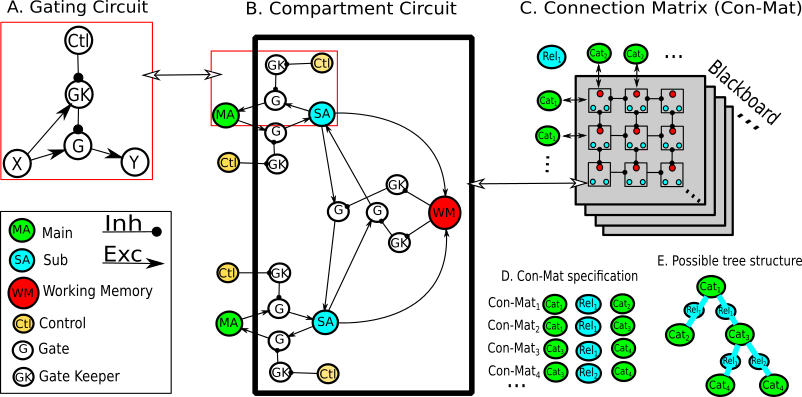
\includegraphics[width=1.00\columnwidth]{figures/part_IV/gating_circuit3}
    \caption{The Neural Blackboard architecture.
      \textbf{A.} Gating circuit that allows the implementation of conditional neural activity transfer between Neural assemblies X and Y through a gate assembly.
      The gate keeper assembly (GK) is activated by the X assembly and then inhibits the gate assembly (G).
      To let information flow through the gate assembly, a control assembly (Ctl) must therefore inhibit the gate keeper assembly.
      \textbf{B.} Architecture of a single compartment circuit of a connection matrix.
      Six gating circuits are arranged in a way that makes conditional bidirectional neural activity flow between two main assemblies possible.
      Control assemblies regulate the direction of information flow and allow the activation of sub assemblies.
      The two sub assemblies excite the working memory assembly which, once activated, encode the binding of the main assemblies and allow activation to flow between them if the controls allow it too.
      \textbf{C.} Each connection matrix contain n by m compartment circuits that encode the same relationship type between the same pair of assembly categories.
      There are $m$ available assemblies for one category and $n$ available assemblies for the complementary category and only one cell circuit can activate its working memory assembly to link two particular assemblies due to mutual row and column inhibition of cells in the connection matrix.
      The size of the connection matrix effectively represents memory limitations.
      A blackboard is composed of an arbitrary number of connection matrices that encode different relationship types for a pair of assembly categories.
      \textbf{D.} A blackboard is composed of multiple connection matrices, where each of them is defined by two node categories and a relationship type between them.
      \textbf{E.} Example of a possible tree structure that can be represented based on the specified connection matrices. }
      \label{Blackboard}
  \end{center}
\end{figure*}


Nodes in Figures {\ref{Blackboard}}.A and {\ref{Blackboard}}.B represent neural assemblies that can be interpreted as linked spiking neural populations.
The most basic component of the NBA is a ``Gating Circuit'' illustrated in Figure {\ref{Blackboard}}.A.
The main idea is that neural activity would flow from the assembly X to the assembly Y, but is blockedby the Gake Keeper (GK) assembly, 
which itself is excited by assembly X.
So to allow directional activity flow from X to Y, a Control (Ctl) assembly has to inhibit the GK assembly.
Notice that it is trivial to extend the gating circuit for bidirectional control of activity flow as illustrated in Figure {\ref{Blackboard}}.B.
Introducing bidirectional conditional control signals is what gives the NBA the possibility of implementing separately queries like 'what follows X?' or 'what follows Y?'.

The second basic component of the NBA is a proposal for working memory (WM).
Persistent neural activity in response to stimuli is considered to be the neural process underlying active (working) memory, and its implementation is hypothesized to be based on excitatory reverberation\citep{wang2001synaptic}.
Based on this, the NBA considers a Delay Activity\citep{de_Kamps_2005} mechanism as a biologically plausible implementation of WM. It consists on a neural assembly, that after being excited beyond a certain threshold, achieved by the coactivation of input populations, will maintain a constant amount of activation for a short period of time. By maintaining its activity, WM acts as a short lived bidirectional link between two assemblies. This mechanism can be considered as the creation of an implicit pointer from one assembly to the other, such that future reactivation of one assembly can be driven from the other to perform query operations. This conforms a ``Memory Circuit'' as depicted in Figure {\ref{Blackboard}}.B.

Two bidirectional ``Gating Circuits'' connected by a ``Memory Circuit'' form a ``Compartment Circuit'' capable of implementing variable binding and query operations.
The key point of this circuit is that Main assemblies (MA), representing grounded concepts or instances of variables types, activate Sub assemblies (SA) 
if a control signal driven by another mechanism allows it.
Then coactivation of SAs is what realizes a temporary binding of MAs by activating WM.
So one ``Compartment Circuit'' models specifically the neural activity of a variable binding operation.
It is operated by a mechanism that drives control signals simultaneously in multiple ``Compartment Circuits'' to instantiate binary tree like data structures on which query/unbinding operations can be performed later. 

As might be evident by now, applying the NBA to syntactic processing in language consists of two simple assumptions.
First, equating the parsing mechanism to the control mechanism that coordinate binding events of words and word types and phrase types.
Second, determining the number of compartment circuits necessary to instantiate a complete syntactic structure and the content of MA nodes from a grammar theory.
In this work we will only employ a phrase grammar and bottom-up parsing scheme following theoretical assumptions of selected neuroimaging experiments.
Nonetheless, a promising feature of the NBA is that it has the flexibility to test any arbitrary parsing mechanism incorporating top-down considerations and an important variety of alternative theories of grammar based on binary trees.
For example dependency grammars that assume multiple direct word bindings instead of the hierarchical phrase bindings modelled in this work have been employed in previous simulations\citep{van_der_Velde_2010}.

To understand how a sentence is processed in the NBA, let us consider first the simplest case of binding two words, like ``Sad student'', 
belonging to grammatical categories instantiated in the MAs of one ``Compartment Circuit'', such that one MA is an ``Adjective'' corresponding to ``sad'' and the other one 
is a ``Noun'' corresponding to ``student''.
The MAs activate with timings corresponding to word presentation, so we are assuming that words were recognized to motivate their corresponding instantiated grammatical 
categories before we attempt to link them.
Then an assumed parsing mechanism determines that a link operating on ``Adjective'' and ``Noun'' types is necessary in the blackboard, driving activity in several 
``Compartment Circuits'' from which only one, that we consider as the recruited ``Comparment Circuit'', completes coactivation of SAs to drive WM and realize binding between the word types.

In the case of a complete phrase, like ``Fat sad student'', if we are assuming the instantiation of phrase types that form a hierarchical tree theorized by a phrase grammar, 
then the time at which the binding of the instantiated grammatical categories of ``sad student'' takes place would be the time at which a ``Noun Phrase'' is activated and bound 
to the ``Adjective'' corresponding to ``Ten''.

Finally, a ``Connection Matrix'', portrayed in Figure {\ref{Blackboard}}.C, allows the implementation of a complete ``Blackboard''.
It contains variable type relations learned by the ``Blackboard'' as sets of mutually inhibitory ``Compartment Circuits'' that enable the selection of the 
``Compartment Circuits'' requested by the control mechanism.
We portray the ``Blackboard'' as a regular grid for illustrative purposes, although there is already a proof of concept implementation with 
randomly connected networks\citep{van_der_Velde_2011}.
Also implementing a general syntactic control mechanism should be feasible. As suggested by the Feed-forward artificial 
neural networks employed in previous NBA simulations~\citep{van_der_Velde_2010} and recent state of the art feedforward network architectures that have shown top performance for diverse language parsing tasks~\citep{andor2016globally}.
Moreover a more recent proposed extension of the NBA, that imitates the motor circuit of the marine mollusk Tritonia diomedea, 
shows how to generate patterns for sequential activation control\citep{van_Dijk_2015}.
Simulating these higher level mechanisms is a task out of the scope of this work, since we focus specifically on reproducing the neural signatures of variable binding operations.
